\chapter{Evaluation}

This chapter presents an evaluation and discussion of the performance and energy efficiency
of the proposed bitcoin mining system.

\section{Measuring Mining Performance}

In order to estimate the bitcoin mining performance of the system, a benchmark is used to
measure the number of double hashes that can be performed each second.
This is done by repeatedly double-hashing a block of data and recording the
number of hashes achieved per second per core. By adding more cores over time, it
is possible to see how the performance scales as more cores are added. Recording
the number of hashes per second per core also makes it possible to see how the performance
of each core is affected by the traffic on the network-on-chip generated by the other
cores in the network. Cores not active are put into a no-operation loop.

Using the architecture setup described in section \ref{sec:SHMAC_sys_arch}, tests where run using the
following method:

\begin{enumerate}
    \item Hashing using software only, not using the SHA-256 hashing module or DMA module.
    All work is done by the on-tile processor.
    \item Hashing using only the hashing accelerator.
    The processor controls and copies data to and from the hashing module.
    \item Hashing using the hashing accelerator and DMA.
    The processor controls each module, but the DMA handles data transfer.
\end{enumerate}

Interrupts are used by the hashing module to signal when it is finished working. However,
%the DMA does not support interrupts and has to be polled while copying data to and from
the software does not support interrupt from DMA, and it has to be polled while copying data to and from
the module, which may have a minor influence on the results.

The benchmark software was compiled using the GCC compiler, version 4.8.2, compiled for
the arm-none-eabi target triplet. To generate a binary file for the SHMAC, utilities
from GNU Binutils version 2.24, also compiled for the arm-none-eabi target triplet,
were used.

\section{Estimating Power Usage}
\label{sec:power-measure}

Power usage for the application is determined by measuring the wall-power of the box
that SHMAC is running on both when idle and when running the test applications. The
power usage of the application is then determined using the following formula, where
$P$ is the power in watts:

\[P_{application} = P_{running} - P_{idle}\]

Using the result of the power measurement, the energy efficiency can be obtained as
the number of hashes per second per watt, H/s/W. As watt is defined as joule per second,
J/s, the unit can be rewritten to hashes per joule, H/J.

To obtain the power usage of SHMAC, a Yokogawa WT210 power meter was used to measure
the power drawn by the Versatile Express box from the power socket in the wall while
idle and when running the bitcoin application. This method provides some uncertainty
in the result of the measurements, as the Versatile Express also runs a Linux host
system. It was not possible to obtain power measurements directly from the FPGA running
SHMAC. % Cannot find a source for the power measurement instrumentation that is in-the-works.
\todo{Remember to underline this uncertainty in the discussion/evaluation part, since}

% FOLLOWING POST-MEETING:
%
%Optional: Write the expected max performance if we can calculate them?
%
%\section{Known hazards with SHMAC and test setup}
%List up potential problems that SHMAC may give us, due to the known bugs in the system (cache coherency issues with DMA, the infamous cache bug.
%
%Also include the uncertainty with testing of wall-power, and the lack of on-chip power measurement.
%
%\section{Tools and software used for this project}
%- Modelsim?
%
%\subsection{Other properties of Vexpress}
%FIND: DDR MEMORY LATENCY AND THROUGHPUT IF POSSIBLE.
%Throughput according to Asbjørn: 128-bit word per cycle.
%Clock is a 50MHz.

\section{Performance Results}

To establish a baseline for the performance gains obtained when using the accelerators,
a measurement of the performance when using software hashing was first obtained. The
performance is measured in the number of double hashes per second and abbreviated H/s,
as is the convention for bitcoin mining systems.

\subsection{Initial Results}
\label{sec:init-results}

Using software-only hashing produced a best result of 21~261~H/s when running with only 4 active processors. As can be seen
in the plot in figure \ref{fig:sw-scaling1}, it can be observed that adding more processors after the fourth produces no
noticeable additional performance gain. The reason for this is that all cores makes frequent
accesses to DRAM, when running the software algorithm, which causes the DRAM tile to quickly
become congested. The reason for these frequent accesses is probably due to the use of
many variables in the code as well as the effect of stack usage. Since the Turbo Amber core
uses a write-through cache, all memory writes ends up going to DRAM immediately which causes
additional congestion.

Another interesting effect to note in the results is how the XY routing affects the performance
of each tile. The more tiles that tries to access main memory through a tile, the less
performance that tile has; network congestion does, in other words, have a great impact on individual
tile performance.

This was especially obvious for processor tile 10, which is located on the end of row 3 with no
processors on either the left or right sides. This processor showed notably better performance than
any other processor in the grid. This is because its location means that no data to or from other processors
have to pass through the processor which gives it more time to process its own requests. In addition,
this processor can access all memory tiles without having to send or receive data through any other
processor tiles because of its location. The individual performance of each processor is noted in
appendix \ref{app:performance}, table \ref{tab:Full-Perf-SW1}.

\begin{figure}
	\centering
	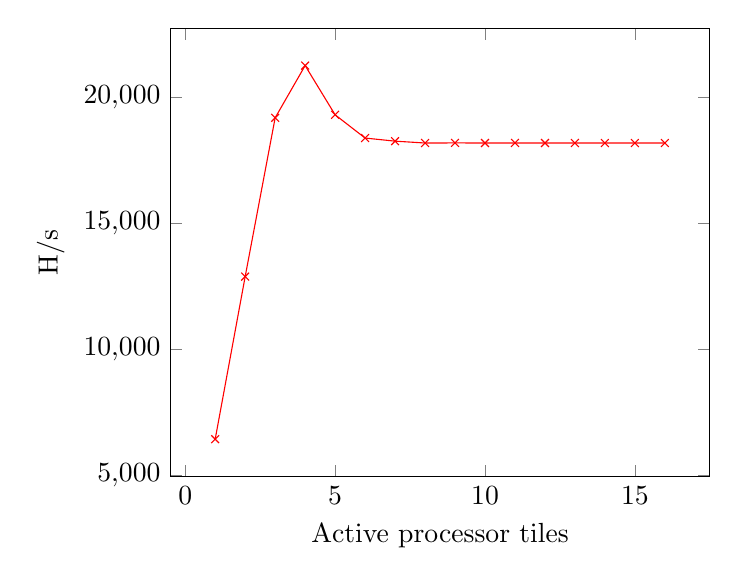
\begin{tikzpicture}
		\begin{axis}[
			xlabel=Active processor tiles,
			ylabel=H/s,
			scaled ticks=false]
		\addplot[color=red,mark=x] coordinates {
		        (1, 6450)
			(2, 12895)
			(3, 19190)
			(4, 21261)
			(5, 19310)
			(6, 18388)
			(7, 18265)
			(8, 18191)
			(9, 18195)
			(10, 18192)
			(11, 18194)
			(12, 18192)
			(13, 18192)
			(14, 18191)
			(15, 18191)
			(16, 18191)
		};
		\end{axis}
	\end{tikzpicture}
	\caption{Software performance}
	\label{fig:sw-scaling1}
\end{figure}

Figure \ref{fig:shadmacomp-scaling1} shows the results when using the SHA-256 accelerator, without and with the DMA module enabled, respectively
Looking at the case where only one core is running, one can see that the performance when using the accelerator and DMA is about 2,8 times faster than
using the software version, at 18~230~H/s in hardware and 6~450~H/s in software. Adding more processors gives an even higher gain due to the
near linear scaling of the performance when using the hardware accelerators.

Only up to four processors where used for this test, as adding in processors from the second row of processors when scaling up caused the application to crash.
An attempt at starting processors from the top and bottom row at the same time also led to a crash.
It was discovered that this was likely because of an bug in the implementation of the scratchpad memory tile used. An attempt was made at integrating fixes
to the scratchpad bug from an experimental SHMAC branch, but failed due to differences in the code. Because of this bug, it is not
possible to predict how many cores can be active and hashing using hardware acceleration at the same time before reaching the memory congestion limit,
nor is it possible to see if the DMA has any significant effect on the performance. It was decided to attempt to work around the scratchpad bug with
a new design, in order to better measure how the performance and energy efficiency of hardware hashing scales and what effect using a DMA will have when more tiles are active.

\begin{figure}
	\centering
	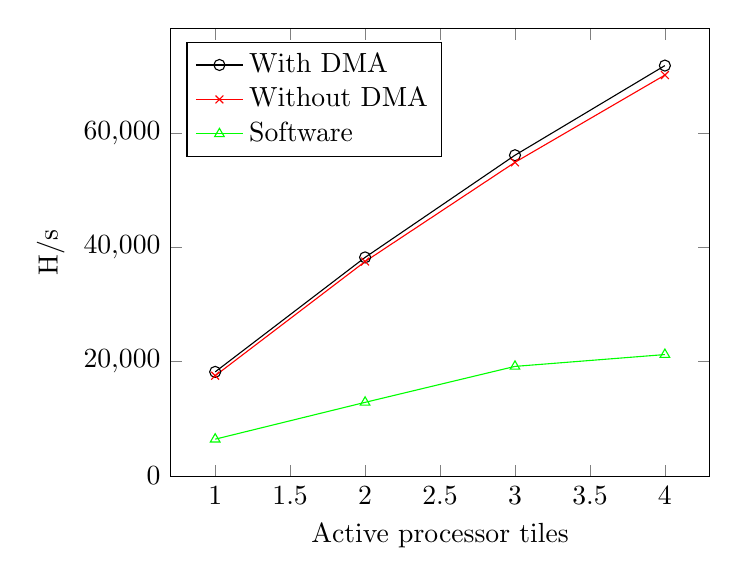
\begin{tikzpicture}
		\begin{axis}[
			xlabel=Active processor tiles,
			ylabel=H/s,
			scaled ticks=false,
			legend pos=north west,
			legend cell align=left]
		\addplot[color=black,mark=o] coordinates {
			(1, 18230)
			(2, 38267)
			(3, 56150)
			(4, 71840)
		};
		\addlegendentry{With DMA}
		\addplot[color=red,mark=x] coordinates {
			(1, 17557)
			(2, 37539)
			(3, 54912)
			(4, 70179)
		};
		\addlegendentry{Without DMA}
		\addplot[color=green,mark=triangle] coordinates {
		        (1, 6450)
			(2, 12895)
			(3, 19190)
			(4, 21261)
		};
		\addlegendentry{Software}
		\end{axis}
	\end{tikzpicture}
	\caption{Hardware hashing performance, with software performance added for comparison}
	\label{fig:shadmacomp-scaling1}
\end{figure}

\subsection{Results from the Alternative Design}
In order to obtain better results with regards to scaling, a new test design was created which works
around the scratchpad tile bug and places 14 CPU cores on the same line in the grid. The design
is described in section \ref{sec:SHMAC_sys_arch}. The performance obtained using only software hashing
is plotted in figure \ref{fig:sw-scaling2} and mirrors the results obtained from the original design,
in that adding more cores after the fourth does not provide any additional performance. The greatest
performance obtained using software hashing in the alternative design was 21~364~H/s with 4 cores
active.

\begin{figure}
	\centering
	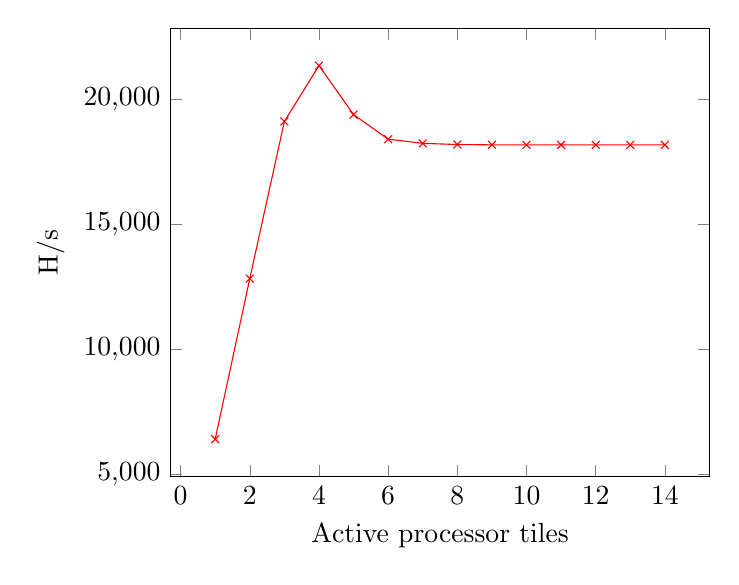
\begin{tikzpicture}
		\begin{axis}[
			xlabel=Active processor tiles,
			ylabel=H/s,
			scaled ticks=false]
		\addplot[color=red,mark=x] coordinates {
		    (1, 6418)
			(2, 12841)
			(3, 19130)
			(4, 21364)
			(5, 19404)
			(6, 18420)
			(7, 18253)
			(8, 18206)
			(9, 18193)
			(10, 18192)
			(11, 18192)
			(12, 18192)
			(13, 18191)
			(14, 18190)
		};
		\end{axis}
	\end{tikzpicture}
	\caption{Software hashing performance for the alternative hardware design}
	\label{fig:sw-scaling2}
\end{figure}

The performance results obtained using the hardware modules are plotted in figure \ref{fig:shadmacomp-scaling2}.
From these results, it can be observed that the performance continues to scale almost linearly up until around
the tenth core is added. At this point, memory congestion is starting to affect the scaling, causing it to
flatten out. The best performance was obtained when running with all cores active, at 175~711~H/s with DMA
enabled or 179~526~H/s with the DMA disabled. Even though this case did not show any advantage of using the
DMA, using the DMA for data transfer \emph{does} provide a small and consistent performance increase when using less than 
12 cores.

The reason for this is that when the CPU is loading data into the hashing accelerator, it first loads
data from main memory into its data cache. This is done using 128-bit transfers, transferring an entire
cache line at a time from the memory. The DMA does, however, only use 32-bit transfers, causing four times
more traffic in the tile network. The speedup observed while using the DMA is likely because the CPU has more
overhead when copying the data from its cache to the accelerator than has the DMA.

\begin{figure}
	\centering
	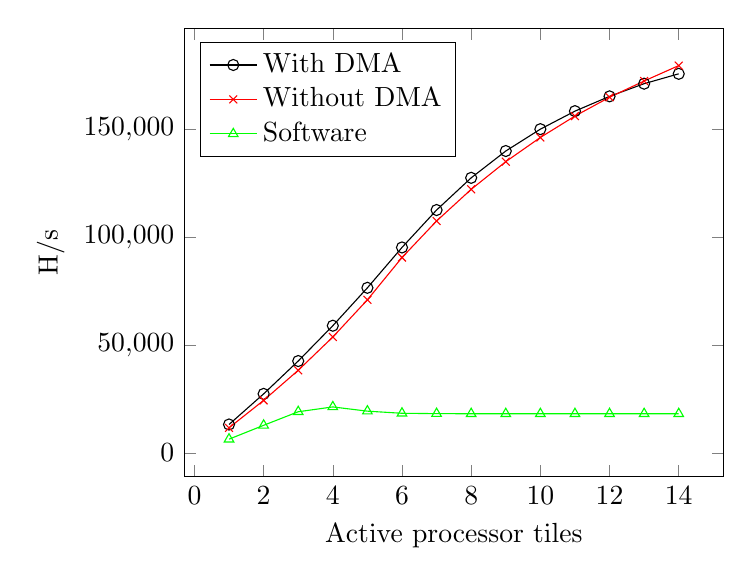
\begin{tikzpicture}
		\begin{axis}[
			xlabel=Active processor tiles,
			ylabel=H/s,
			scaled ticks=false,
			yticklabel style={/pgf/number format/fixed},
			legend pos=north west,
			legend cell align=left]
		\addplot[color=black,mark=o] coordinates {
			(1, 13227)
			(2, 27410)
			(3, 42627)
			(4, 58989)
			(5, 76556)
			(6, 95259)
			(7, 112599)
			(8, 127515)
			(9, 139937)
			(10, 150069)
			(11, 158421)
			(12, 165271)
			(13, 171143)
			(14, 175711)
		};
		\addlegendentry{With DMA}
		\addplot[color=red,mark=x] coordinates {
			(1, 11676)
			(2, 24394)
			(3, 38329)
			(4, 53760)
			(5, 70983)
			(6, 90590)
			(7, 107510)
			(8, 122186)
			(9, 135009)
			(10, 146221)
			(11, 156133)
			(12, 164860)
			(13, 172381)
			(14, 179526)
		};
		\addlegendentry{Without DMA}
		\addplot[color=green,mark=triangle] coordinates {
		    (1, 6418)
			(2, 12841)
			(3, 19130)
			(4, 21364)
			(5, 19404)
			(6, 18420)
			(7, 18253)
			(8, 18206)
			(9, 18193)
			(10, 18192)
			(11, 18192)
			(12, 18192)
			(13, 18191)
			(14, 18190)
		};
		\addlegendentry{Software}
		\end{axis}
	\end{tikzpicture}
	\caption{Hardware results for the alternative hardware design with software results added for comparison.}
	\label{fig:shadmacomp-scaling2}
\end{figure}

\section{Power and energy efficiency}

The energy efficiency was calculated by measuring the power usage of the application, as described in section \ref{sec:power-measure},
and looking at how many double hashes the system does. This provides a number of double hashes per second per watt.

Obtaining the power measurements provided a difficult task, as the idle power of the Versatile Express box seemed to be
steadily rising over time. This can be caused by multiple factors, such as the host system working, changes in temperature
due to the benchmark application running or environmental factors. Because of this, the idle power was measured between
each individual test run to make sure the power usage of the application was measured as correctly as possible.

Because of the problems encountered with the initial test design, only the power results from the alternative design
is discussed here. However, both designs show the same trends, and the results from the initial design can be seen in
the appendix, section \ref{sec:energy-initial}.

Figure \ref{fig:power-plot} shows the measured power usage when running with software hashing, accelerated hashing without DMA
and accelerated hashing with DMA.

\begin{figure}
	\centering
	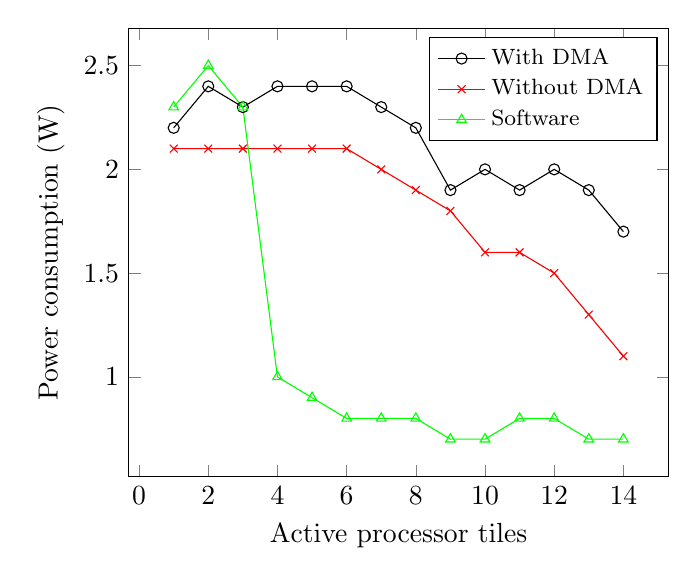
\begin{tikzpicture}
		\begin{axis}[
			xlabel=Active processor tiles,
			ylabel=Power consumption (W),
			legend cell align=left,
			legend style={font=\footnotesize},
			scaled ticks=false]
		\addplot[color=black,mark=o] coordinates {
			(1, 2.2)
			(2, 2.4)
			(3, 2.3)
			(4, 2.4)
			(5, 2.4)
			(6, 2.4)
			(7, 2.3)
			(8, 2.2)
			(9, 1.9)
			(10, 2.0)
			(11, 1.9)
			(12, 2.0)
			(13, 1.9)
			(14, 1.7)
		};
		\addlegendentry{With DMA}
		\addplot[color=red,mark=x] coordinates {
			(1, 2.1)
			(2, 2.1)
			(3, 2.1)
			(4, 2.1)
			(5, 2.1)
			(6, 2.1)
			(7, 2.0)
			(8, 1.9)
			(9, 1.8)
			(10, 1.6)
			(11, 1.6)
			(12, 1.5)
			(13, 1.3)
			(14, 1.1)
		};
		\addlegendentry{Without DMA}
		\addplot[color=green,mark=triangle] coordinates {
			(1, 2.3)
			(2, 2.5)
			(3, 2.3)
			(4, 1.0)
			(5, 0.9)
			(6, 0.8)
			(7, 0.8)
			(8, 0.8)
			(9, 0.7)
			(10, 0.7)
			(11, 0.8)
			(12, 0.8)
			(13, 0.7)
			(14, 0.7)
		};
		\addlegendentry{Software}
		\end{axis}
	\end{tikzpicture}
	\caption{Measured power consumption using software and hardware accelerators.}
	\label{fig:power-plot}
\end{figure}

For software-only hashing, it is interesting to note that less power is used when adding more cores. With 1--3 cores
active, the power usage for the application was measured to be between 2,3~W and 2,5~W, while running at 5 cores and
more only used between 0,7~W and 0,8~W.

One reason for this may be that as more tiles are added, longer periods of stalling is needed for each core to wait for data from
the main memory. When cores are inactive, they are waiting in a nop-operation loop, a software loop consisting of a
\textsc{nop} operation. Executing this loop causes the processor to have to decode and execute two instructions,
the no-operation instruction and the branch instruction. However, when stalling, the processor does not decode or
execute new instructions, which may cause less switching to happen internally in the processor, thus reducing power
wasted from transistor switching. This could be a good indicator that the Turbo Amber processor could benefit
from a form of sleep or wait-for-interrupt instruction, which is not currently supported by the processor \cite{amber-spec}, that will
allow it to stall as long as it has no work to do.

The same trend can be seen when using hardware, although the drop in power usage is not as pronounced as in the software-only
case . This is likely because it takes longer for the traffic to the memories to be large enough to cause longer periods of
stalling in the processor and DMA module.

The energy efficiency is shown in figure \ref{fig:efficiency-plot}. It is evident that using a hardware accelerated
hashing module provides large gains in energy efficiency, which becomes especially clear when adding more than 4 cores,
because of the much higher performance the accelerators can provide with little overhead in energy use. At 14 active
tiles, hardware acceleration without DMA provides over 6 times better energy efficiency than software hashing,
at 163~205,5~H/J versus 25~985,5~H/J.

It is interesting to note that the energy efficiency when using a DMA becomes notably worse than when the DMA is disabled
when the interconnect network is starting to become congested, around the point where 10 cores and more are active.

\begin{figure}
	\centering
	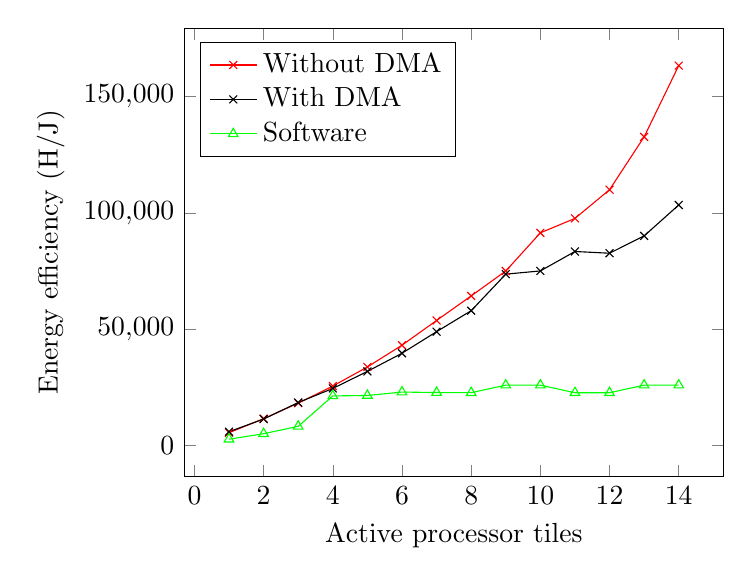
\begin{tikzpicture}
		\begin{axis}[
			xlabel=Active processor tiles,
			ylabel=Energy efficiency (H/J),
			yticklabel style={/pgf/number format/fixed},
			legend pos=north west,
			legend cell align=left,
			scaled ticks=false]
		\addplot[color=red,mark=x] coordinates {
			(1, 5560)
			(2, 11616.2)
			(3, 18251.9)
			(4, 25600)
			(5, 33801.4)		
			(6, 43138.1)
			(7, 53755)
			(8, 64308.4)
			(9, 75005)
			(10, 91388.1)
			(11, 97583.1)
			(12, 109906.7)
			(13, 132600.8)
			(14, 163205.5)
		};
		\addlegendentry{Without DMA}
		\addplot[color=black,mark=x] coordinates {
			(1, 6012.3)
			(2, 11420.8)
			(3, 18533.5)
			(4, 24578.8)		
			(5, 31898.3)
			(6, 39691.3)
			(7, 48956.1)
			(8, 57961.4)
			(9, 73651.1)
			(10, 75034.5)
			(11, 83379.5)
			(12, 82635.5)
			(13, 90075.3)
			(14, 103359.4)
		};
		\addlegendentry{With DMA}
		\addplot[color=green,mark=triangle] coordinates {
			(1, 2790.4)
			(2, 5136.4)
			(3, 8317.4)
			(4, 21364)
			(5, 21560)
			(6, 23025)
			(7, 22816.3)
			(8, 22757.5)
			(9, 25990)
			(10, 25988.6)
			(11, 22740)
			(12, 22740)
			(13, 25987.1)
			(14, 25985.7)
		};
		\addlegendentry{Software}
		\end{axis}
	\end{tikzpicture}
	\caption{Energy efficiency}
	\label{fig:efficiency-plot}
\end{figure}

The numbers obtained here shows that our accelerated hashing tile cannot compete with other FPGA-based bitcoin hashing systems,
such as BTCMiner, mentioned in section \ref{sec:fpga-mining}, which gets a result of 21~MH/J as opposed to our 163,3~kH/J.
There are several reasons for this, mainly the lack of pipelining in the SHA-256 accelerator, which slows throughput by 65 times
compared to a fully unrolled SHA-256 pipeline.

%\section{Discussion about NoC efficiency}

% Relevant stuffz copied from methodology:
%
%Caches were turned on for each testing, but a bug in the caches can cause several processors to halt over time, making measurements more difficult.
%Increased number of tiles in used increases the chance for a cache bug to happen.
%Additionally, no cache coherency protocol is implemented, and all shared data are therefore mapped to uncachable memory.
%Data hazard may be present when DMA and processor "shares" data, by loading or storing to the same address space in use.
%DMA may copy outdated data from memory that the cache has not yet written back, or overwrite data that the cache is not aware of.
%An operating system may handle data coherency where DMA involved, but since this project is done by running the software on bare metal, this security is absent.
%The Turbo Amber processor uses \todo{Must get it confirmed, and then source linked}write-through policy, so every data update is always written back to memory, \todo{Want to mention "reduced, but not removed", due to how our tests may go} reducing the possibility of data hazard, but not removing it.

%Interrupt handling for the hashing module is always in use, when the accelerator is used.

%The DMA Module is made only for transfering 32-bit words individually at a time.
%When transferring data internal on the tile (regular tile registers, hashing registers and DMA registers), this is all the local system requires, as the tile modules does not provide full blocks of \todo{Use of wishbone, with size 128, is not yet provided}4 words.
%\todo{Merely an assumption. We haven't tested this.}But when running the hashing in software only, the system is likely to achieve better data transfer rate using regular processor data transfer of 4 words, through the caches, since the current DMA would require 4 individual transfer, compared to the processor.

%The use of the included sub-module in the DMA that moves the bytes from high endian to little endian should further improve the performance and energy efficiency, by relieving the software for this task.
%The byte flip is done through combinatorical circuits, and should not add any extra execution time.
%Wihtout it, the software would require several independent operations, for loading in and shifting every single byte to the correct position of the word.

%Additionally, polling is used to control when a DMA is finished.
%Ideally, interrupt handling is preferable, but the interrupt handler for the DMA would not \todo{yet}work. 

